\documentclass[oneside]{book}
\usepackage[utf8]{inputenc}
\usepackage{float}
\usepackage{graphicx}
\usepackage{amsmath}
\usepackage{color}
\usepackage{multicol}
\usepackage{ragged2e}
\usepackage{listings}
\usepackage{pdfpages}
\title{Notes de Cours INF 3610}
\date{2018-10-10}
\author{Olivier Sirois}
\setlength\parindent{0pt}
\makeindex
\pagenumbering{arabic}
\begin{document}
    \setcounter{page}{1}
    \maketitle
    \tableofcontents
    \chapter{Chapitre 1 - Introduction}
    On peu définir la vérification formelle comme étant l'utilisation de techniques théorique pour prouver le fonctionnement d'un système. Selon Sommerville, la vérification est la réponse à la question:\\
    %%\centering
    \textbf{Are we building the product right}\\
    
    Pour etre vérifié, un système doit satisfaire:
    \begin{itemize}
        \item Vérification formele complète : exploration de façon exhaustive de tous les états possible du système
        \item Vérification formelle incomplète : vérification des bornes
    \end{itemize}

    \begin{figure}[!ht]
    	\centering
    	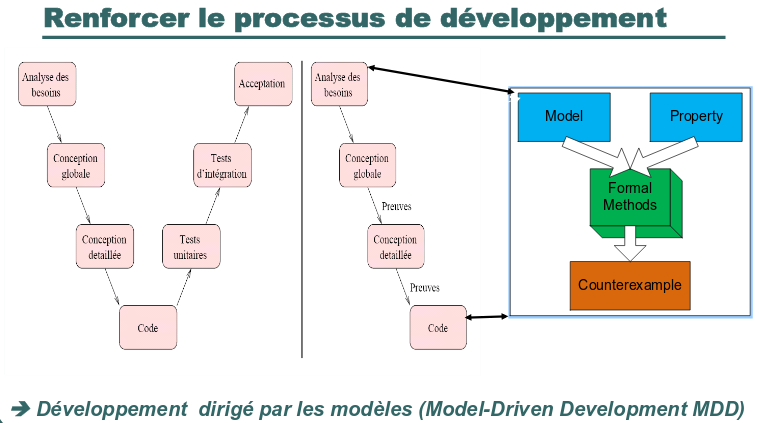
\includegraphics[width = 7cm, height = 7cm, keepaspectratio]{Images/processus_de_developpement.png}
    	\caption{Processus de Développement}
    	\label{fig:ProcessusDeveloppement}
    \end{figure}
    On vérifie formellement pour renforcer le processus de développement. Les techniques de vérification peuvent s'appliquer à différent niveau, car on regarde seulement le fonctionne du module sous test, pas tous le système.\\
    
    \begin{figure}[!ht]
    	\centering
    	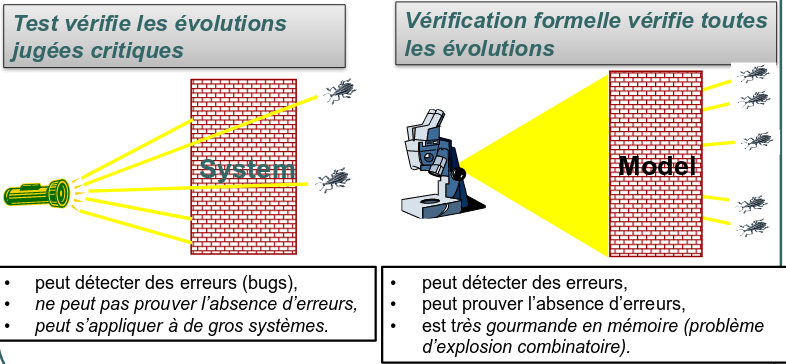
\includegraphics[width = 7cm, height = 7cm, keepaspectratio]{Images/types_tests.png}
    	\caption{Différents types de tests}
    	\label{fig:TypesTests}
    \end{figure}
    
    On voit sur la photo la différence entre les deux méthodes de vérification, une est applicable à un gros système vs. l'autre qui ne peut être fait que sur des éléments de petites tailles.\\
    
    Évidemment, certains accidents notables peuvent être attribuer à un manque de vérification. sa peut aller de AT\&T à la NASA. (problème d'inversion).\\
    
    Lorsqu'on fait affaire dans des systèmes critiques, soit:
    \begin{itemize}
        \item Transport (avionique, ferroviaire, spatial)
        \item Energie (nuclearire...)
        \item Medical (dosage radioactif)
    \end{itemize}

    En raison de la criticalités de ces applications, certains documents ont été mis en place pour la production de logiciel pour les applications aéronautiques.\\
    
    Les normes ED-12C et DO-178C précisent ces contraintes.\\
    
    \subsection{Comment vérifier formellement}
    \begin{itemize}
        \item Modéliser
        \item Spécifier
        \item Prouver
    \end{itemize}

    \begin{figure}[!ht]
    	\centering
    	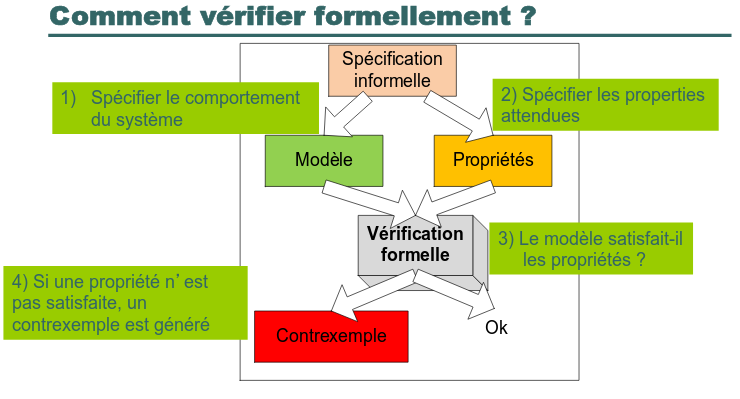
\includegraphics[width = 7cm, height = 7cm, keepaspectratio]{Images/flowchart_verification.png}
    	\caption{Flowchart représentant les étapes de la vérification formelle}
    	\label{fig:FlowchartVerification}
    \end{figure}
    
    \subsection{Comment spécifier un comportement}
    Le but de la modélisation est d'expirmer, au moyen d'un formalisme la manière dont le système se comporte. Le formalisme doit être assez expressif, repose sur une sémantique rigoureuse et doit offrire des possibilités d'analyse systématique. On peut résumé sa en une représentation simplifiée d'un système.\\
    
    Dans le cas des systèmes temps réelles, le fonctionnement est assujetti à l'évolution dynamique de l'environnement et la réaction aux stimuli est soumise à des contraintes temporelles. c-a-d, il faut que la réponse à l'environnement arrive dans un temps spécifier. Plusieurs modèle formels ont été développés puis adaptés aux systèmes temps réel. On peut les distingué par la séquentialité (concurrence), le non-déterminisme, la synchronisation, la communication, la compositionnalité, les contraintes temporelles. On a même certains language de spécifications fait pour pouvoir vérifier des sytèmes.\\
    
    les classe de modèles proposé dans la litérature sont :
    \begin{itemize}
        \item langage de programmation et de spécialisation
        \item les modèles à base de transitions
        \item les modèles logiques
        \item les modèles algébriques
    \end{itemize}
    
    INSÉRÉ SLIDE 27\\
    
    en générales, les modèles doivent spécifier les:
    \begin{itemize}
        \item actions :
        \begin{itemize}
        	\item Déplacement d'un ascenseur
        	\item fermeture de vanne
        	\item Écriture dans une base de donnée
        \end{itemize}
        \item événement:
        \begin{itemize}
        	\item Dépassement d'une température
        	\item Réception d'un message
        \end{itemize}
        \item contraintes temporelle
        \begin{itemize}
        	\item Trouver un vol pour une destination
        	\item envoi de message toutes les 100 secondes
        \end{itemize}
        \item conditions d'activation
        \begin{itemize}
        	\item à respecter avant de déclencher des actions
        	\item s'il n'y a pas d'obstacle devant la cellule de l'ascenseur
        	\item fermer la porte de l'ascenseur
        	\item etc.
        \end{itemize}
        \item situations anormale et leurs traitements
        \begin{itemize}
        	\item arrêt de l'ascenseur entre deux étages
        	\item appui de touche sans résultats
        	\item etc.
        \end{itemize}
        \item les états significatifs
        \begin{itemize}
        	\item ascenseur à l'arrêt
        	\item ascenseur en mouvement
        	\item porte ouverte et ascenseur en mouvement
        \end{itemize}
    \end{itemize} 

    langage de prog -> séparer en deux partie:
    \begin{itemize}
        \item classique, JAVA, C, C++
        \item ceux basé sur un modele de transition, RT-LOTOS, PROMELA, ESTEREL, LUSTRE
    \end{itemize}
    
    \subsection{JAVA}
    
    Java pathfinder, vérificateur (model-checker) pour la NASA. (babelfish). \\
    
    \begin{figure}[!ht]
    	\centering
    	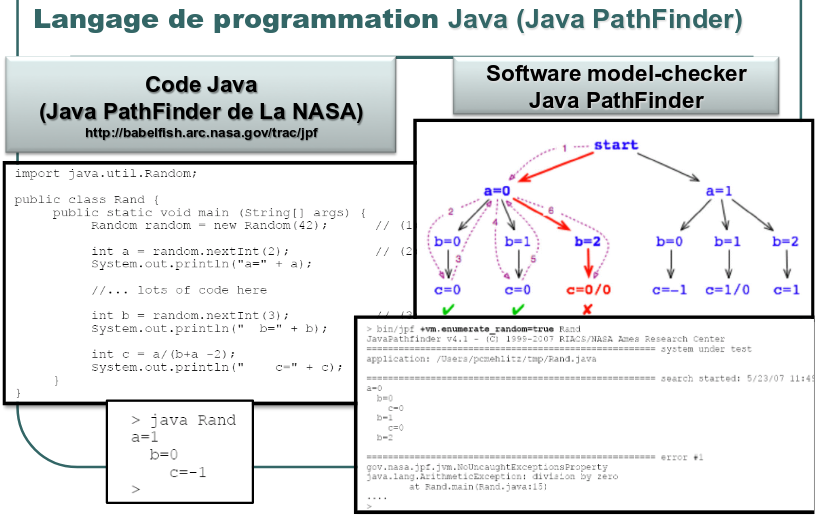
\includegraphics[width = 7cm, height = 7cm, keepaspectratio]{Images/java_pathfinder.png}
    	\caption{flowchart représentant le pathfinder java}
    	\label{fig:JavaPathfinder}
    \end{figure}
    
    \subsection{LLBMC - low level bounded model checker}
    travail sur un code bas niveau (assembleur?). il fait du bounded model-checking dépendament du domaine spécifier.\\
    
    \begin{figure}[!ht]
    	\centering
    	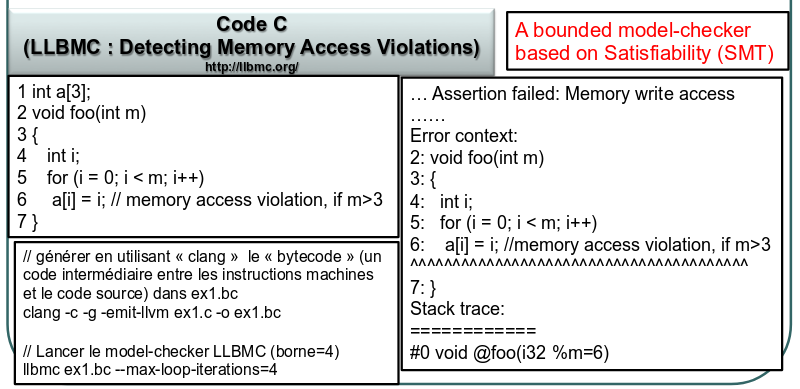
\includegraphics[width = 7cm, height = 7cm, keepaspectratio]{Images/llbmc.png}
    	\caption{Exemple d'utilisation du LLBMC}
    	\label{fig:LLBMC}
    \end{figure}
    
    \subsection{Promela, model-checker SPIN}
    Promela (protocol/process meta language) est utilisé par le model checker SPIN. cré dynamiquement des processus concurrents, la communication entre processus via des variables partagées et des canaux de messages\\
    
    \begin{figure}[!ht]
    	\centering
    	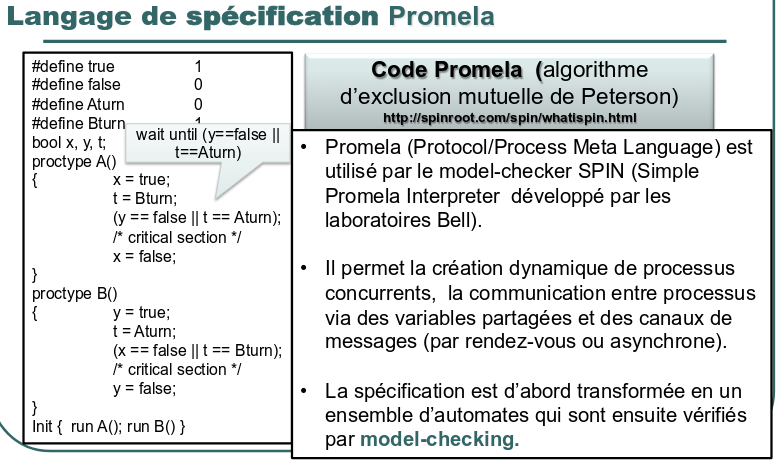
\includegraphics[width = 7cm, height = 7cm, keepaspectratio]{Images/exemple_promela.png}
    	\caption{Exemple d'utilisation de Promela}
    	\label{fig:PROMELA}
    \end{figure}
    
    \subsection{LUSTRE, (boite a outils SCADE)}
    language synchrone a flots de donnees. Sa permet d'exprimer un systeme sour forme d'équations qui définissent l'évolution des valeurs de ses varables\\
    
    Une variable x de LUSTRE représente une flot c-à-d une séquence infinie de valeurs ou x0 est la valeur initiale et xi est la valeur de x au $i^{eme}$ cycle d'exécution.
    
    on peut spécifier un programme aussi comme sur la slide 39\\
    \begin{figure}[!ht]
    	\centering
    	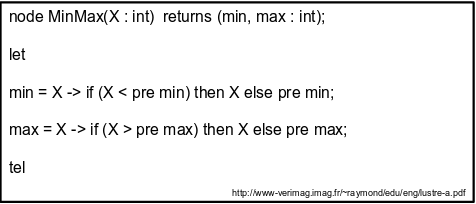
\includegraphics[width = 7cm, height = 7cm, keepaspectratio]{Images/exemple_lustre.png}
    	\caption{Exemple d'utilisation de Lustre}
    	\label{fig:ExempleLustre}
    \end{figure}
    
    \subsection{Modele a base de transition}
    On simule une sorte de state machine mealy, ou on modélise les états discrèt par états ainsi que leur transitions par rapport à leurs actions\\
    
    Ces modèles sont en générales graphique:
    \begin{itemize}
        \item Les Statecharts
        \item Les Ré seaux de Petri
        \item Les Automates
    \end{itemize}

    Les automates offrent un bon compromis entre la puissance de modélisation et la complexité de vérification\\
    
    \begin{figure}[!ht]
    	\centering
    	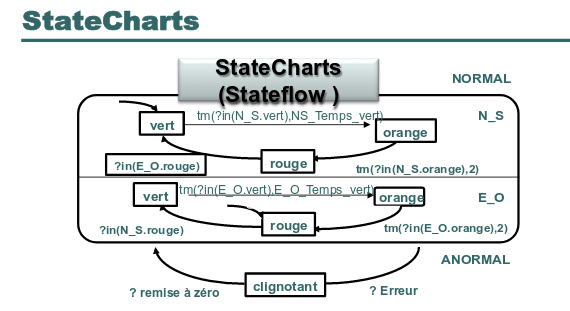
\includegraphics[width = 7cm, height = 7cm, keepaspectratio]{Images/statechart.png}
    	\caption{Exemple d'une statechart}
    	\label{fig:StateChart}
    \end{figure}
	
	\begin{figure}[!ht]
		\centering
		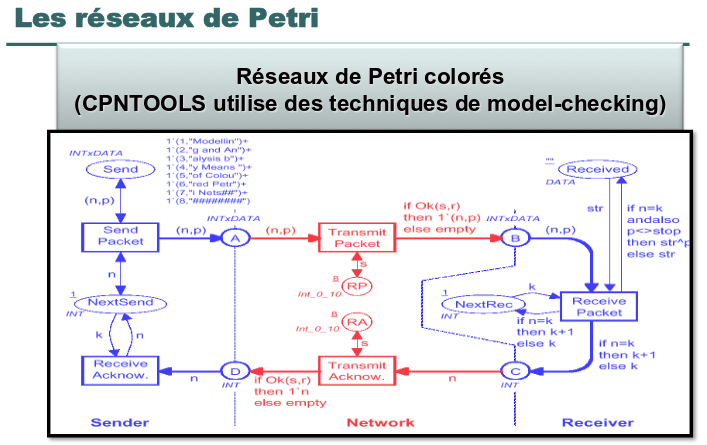
\includegraphics[width = 7cm, height = 7cm, keepaspectratio]{Images/reseaux_petri.png}
		\caption{Exemple d'un réseaux de pétri}
		\label{fig:PetriNetwork}
	\end{figure}

	\begin{figure}[!ht]
		\centering
		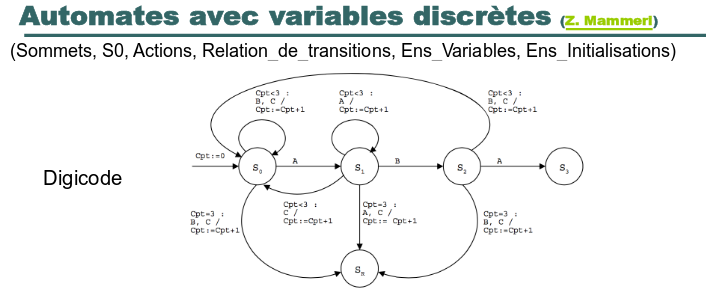
\includegraphics[width = 7cm, height = 7cm, keepaspectratio]{Images/automate_discret.png}
		\caption{Exemple d'un automate avec variables discrèt}
		\label{fig:AutomateDiscret}
	\end{figure}


    
    \subsection{Modeles Logiques}
    
    \begin{figure}[!ht]
    	\centering
    	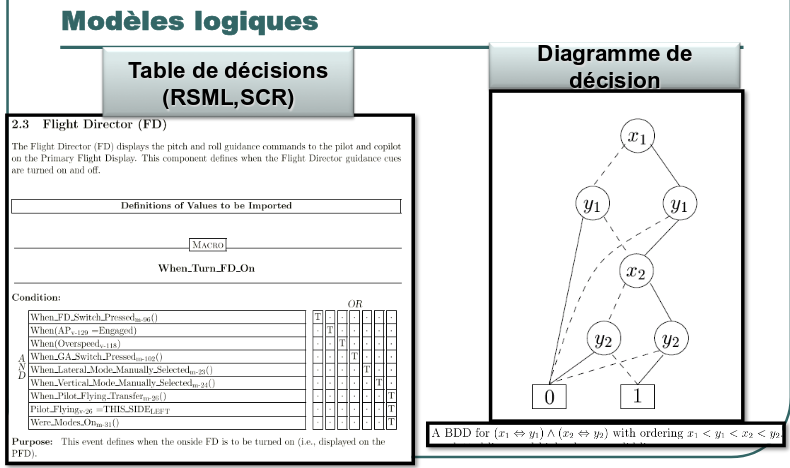
\includegraphics[width = 7cm, height = 7cm, keepaspectratio]{Images/modele_logique.png}
    	\caption{Exemple d'une représentation par modèle logique}
    	\label{fig:ModeleLogique}
    \end{figure}
    
    \subsection{Modèles Algébrique}
    
    Description du comportement d'un système à l'aide d'une description algébrique. On combine des opérateurs et des actions.\\
    \begin{itemize}
    	\item préfixage : $<;>  : a ; C$
    	\item parallèle : $<\lvert\lvert> :C_1 \lvert\lvert C_2$
    	\item choix (non déterministe) $<[]> ou <+> : C_1 []C2$
    \end{itemize}

	l'algèbre des processus CCS et ATP sont dans ces catégories.\\
    
    \subsection{Comment spécifier une proprité}
    On peut utiliser la logique (propositionelle, prédicat), pour spécifier des chose. Sauf que c'étais insuffisant pour décrire des systèmes à comportement temporels. On a alors étendu ces notions à logique temporelle pour pouvoir vérifier formellement des systèmes de natures temporelle.\\
    
    \begin{figure}[!ht]
    	\centering
    	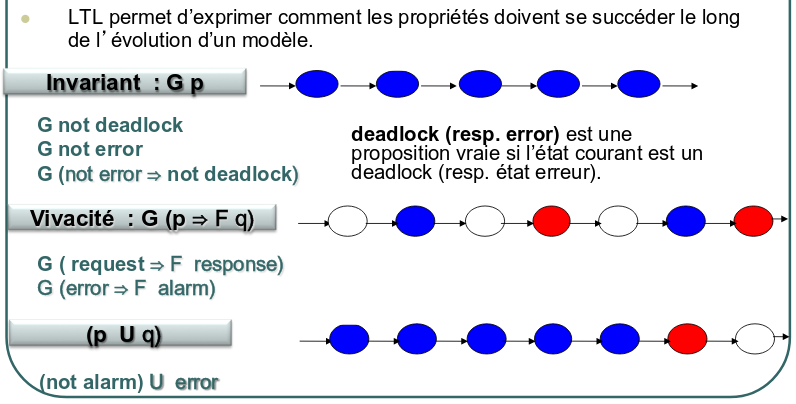
\includegraphics[width = 7cm, height = 7cm, keepaspectratio]{Images/exemple_ltl.png}
    	\caption{Exemple de différentes propriétés de LTL}
    	\label{fig:LTL}
    \end{figure}

    \subsection{Logique temporelle linéaire}
    LTL permet d'expliquer comme la logique évolue dans le temps\\
    
    \subsection{Logique temporelle arborescente (CTL)}
    Cette logique permet de quantifier les chemins d'exécutions\\
    
    \begin{figure}[!ht]
    	\centering
    	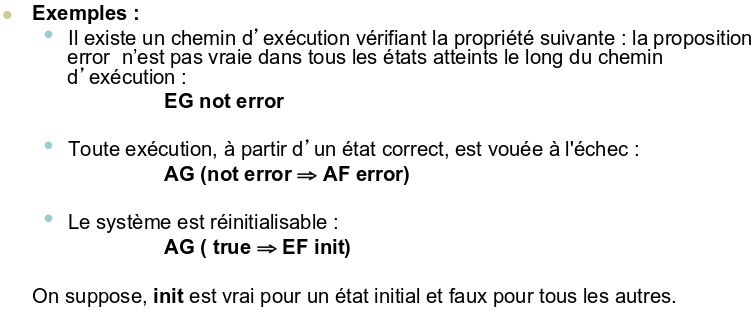
\includegraphics[width = 7cm, height = 7cm, keepaspectratio]{Images/exemple_ctl.png}
    	\caption{Exemple de différentes propriétés de CTL}
    	\label{fig:CTL}
    \end{figure}
    
    
    \subsection{Vérification effective}
    La vérification est dite décidable pour un ensemble de modèles M et une classe de propriétés P si et seulement si il existe un programme qui prend en trné un modèle quelconque de M et une propriété quelconque de P et détermine au bout d'un temps fini, si la propriété est satisfaite ou non par le modèle. Pour être automatisable, la vérification doit être décidable et aussi de complexité acceptable. On différencier entre deux grandes catégories de méthodes: les méthodes syntaxiques et les méthodes sémantiques.\\
    
    \subsection{Méthodes syntaxiques}
    Ce sont des preuves au sens mathématique du terme. Elles cherchent à déterminer si une propriété peut être obtenus.. difficile a automatiser\\
    
    \begin{figure}[!ht]
    	\centering
    	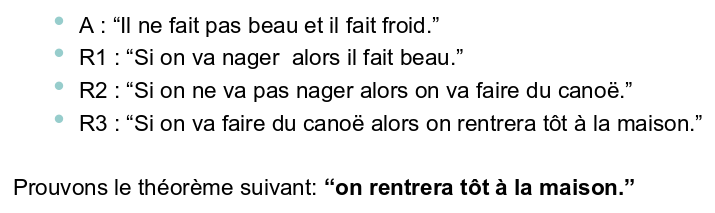
\includegraphics[width = 7cm, height = 7cm, keepaspectratio]{Images/methode_syntaxique.png}
    	\caption{Exemple d'inférence avec la méthode syntaxique}
    	\label{fig:MethodeSyntaxique}
    \end{figure}
    
    Pour résoudre syntaxiquement, on utilise les méthodes vu dans le cours 8215 (logique prédicats/propositionelle)\\
    
    \subsection{Méthodes sémantiques}
    Dans les méthodes sémantiques, on se base sur l'exécution du modèle. L'approche populaire est le model-checking. Sa s'appuie sur deux formalisme:
    \begin{itemize}
        \item système de transition
        \item logique temporelle
    \end{itemize}

    \begin{figure}[!ht]
    	\centering
    	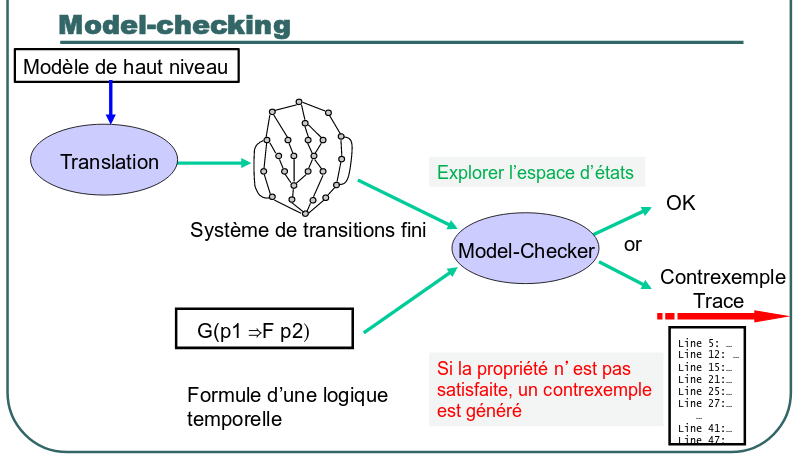
\includegraphics[width = 7cm, height = 7cm, keepaspectratio]{Images/flot_model_checking.png}
    	\caption{Exemple de float à haut niveau de Model-checking}
    	\label{fig:ModelChecking}
    \end{figure}
    
    \subsection{Model-checking}
    Normalement automatique, et produit des contrexemple sous forme de traces qui sont utils à la compréhension des situations d'erreurs et àla correction. basé sur la sémantique d'entrelacement, avec sa, sa pourrait générer n! et plus de $2^{n}$ états\\
    
    Gros problème d'explosion combinatoire avec sa..\\
    
    \chapter{Cours 2 - Automate temporisé}
    \section{Introduction}
    \paragraph{Systèmes temps réel} Agit dans l'environnement.. \\
    \begin{figure}[!ht]
    	\centering
    	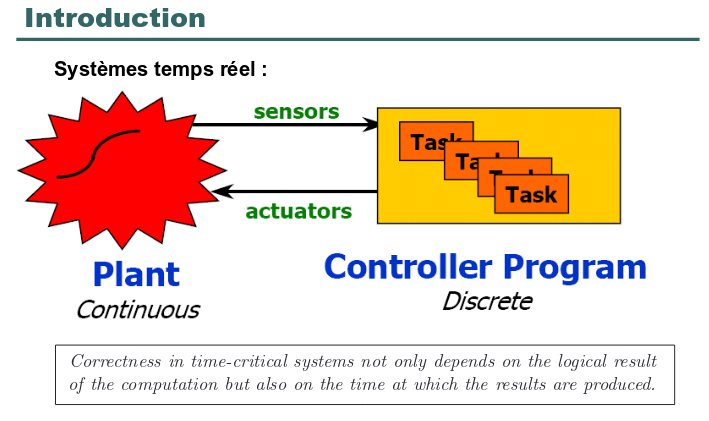
\includegraphics[width = 7cm, height = 7cm, keepaspectratio]{Images/real_time_systems.png}
    	\caption{Concept de système temp réel}
    	\label{fig:RealTimeSystems}
    \end{figure}
    
    Normalement, le systèmes captes son environnement à l'aide de \textbf{capteurs}, fait des traitements (normalement dans un temps définis) et agit ensuite dans son environnement à l'aide d'\textbf{actuateurs}.\\
    
    Le principe est que dans un système temps réel, on doit répondre dans un temps requis. La vérification de tels systèmes doivent alors prendre en considération les contraintes temporelles.\\
    \begin{itemize}
        \item Statecharts, réseaux de pétri temporisé, Automates temporisés
        \item Algèbre de processus temporisé
        \item language synchrone
    \end{itemize}
    \textbf{Automates temporisé}: offrent un très bon compromis entre la puissnace de modélisation et la complexité de vérification.\\
    
    \begin{figure}[!ht]
    	\centering
    	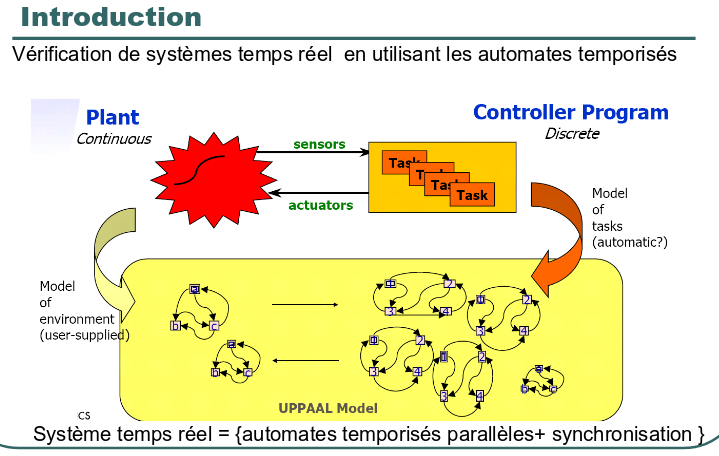
\includegraphics[width = 7cm, height = 7cm, keepaspectratio]{Images/rtsys_environnement.png}
    	\caption{Système temps réel dans l'environnement}
    	\label{fig:RTSYSInEnv}
    \end{figure}
    
    De plus, on ne peut pas se contenter de simplement modéliser le System under test, on doit aussi modéliser l'environnement et ses interactions avec le systèmes testé.\\
    
    \section{Automates}
    un automate est un tuple A = < L, Act, E, I0> ou:
    \begin{itemize}
        \item L est un ensemble fini et non vide de sommets (locations)
        \item Act est un ensemble fini d'actions pour le sommet
        \item E $\in$ L x Act x L est un ensemble fini de transition possible (transitions)
        \item I0 est 'état initiale
    \end{itemize}

    \begin{figure}[!ht]
    	\centering
    	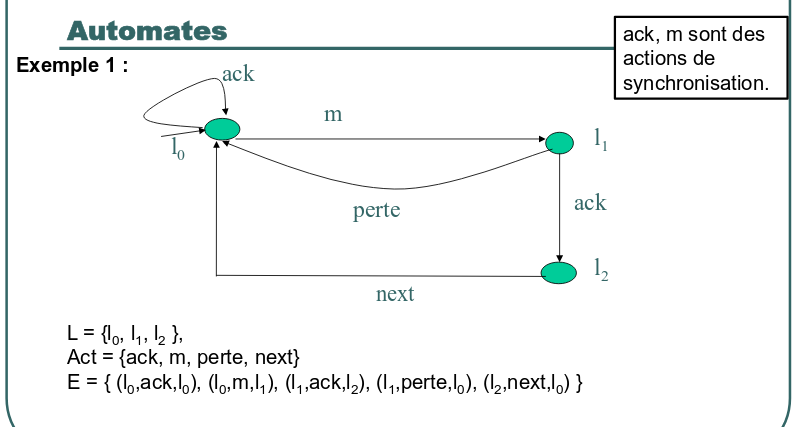
\includegraphics[width = 7cm, height = 7cm, keepaspectratio]{Images/automate_simple.png}
    	\caption{Exemple initiale d'automate}
    	\label{fig:AutomateSimple}
    \end{figure}
    
    d'un automate, on peut extraite un évolution. Qui est une séquence alterné d'états et d'actions. Il est possible de déduire les évolutions possible du modèles. On appelle trace d'exécution la séquence d'action exécutées selon une évolution. ex: action1 -> action2 -> action3.\\
    
    Avec deux automates, leurs composition est le produit scalaire entre les deux automates:
    \begin{itemize}
    	\item $A_1 \lvert\lvert A_2 = <L_1 x L_2, Act_1 \cup Act_2, E, (I_{01},I_{01})>$ ou
    	\item E $\subseteq$ $(L_1 x L_2) x (Act_1 \cup Act_2) x (L_1 x L_2)$ et
    	\item $((I_1, I_2), a, (I_1', I_2')) \in E$ ssi
    	\begin{itemize}
    		\item a $\in$ $Act_1 - Act_2$ $\land$ $(I_1, a, I_1')$ $\in$ $E_1$ $\land$ $I_2=I_2'$ $\lor$
    		\item a $\in$ $Act_2 - Act_1$ $\land$ $(I_2, a, I_2')$ $\in$ $E_2$ $\land$ $I_1=I_1'$ $\lor$
    		\item a $\in$ $Act_1 \cap Act_2$ $\land$ $(I_1, a, I_1')$ $\in$ $E_1$ $\land$ $(I_2, a, I_2')$ $\in$ $E_2$
    	\end{itemize}
    \end{itemize}
    
    \begin{figure}[!ht]
    	\centering
    	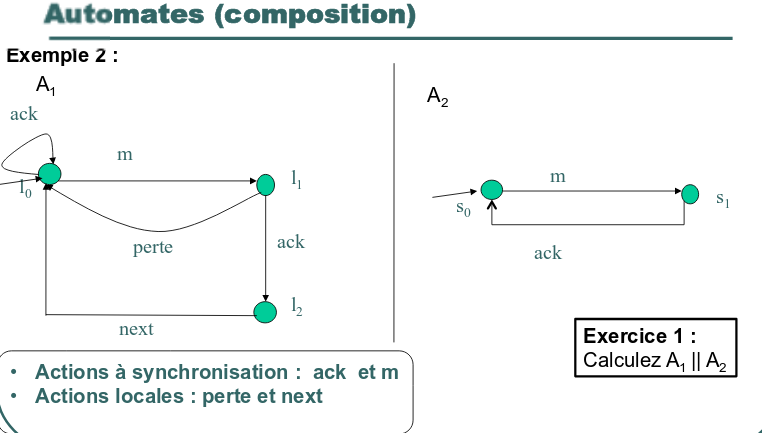
\includegraphics[width = 7cm, height = 7cm, keepaspectratio]{Images/composition_automate.png}
    	\caption{Exemple d'une composition de deux automates}
    	\label{fig:CompositionAutomate}
    \end{figure}
    
    représentent le produit entre deux automates. Il prend en compte des actions des deux automates (synchronisation) versus les actions locals à chaque automates.\\
    
    
    
    
    \section{Automates Temporisé}
    On peutrajouter des contraints temporelles. Lorsqu'un message m est émis, m est déclaré perdu si aucun acquitetement n'est recu avant les 5 unités de temps qui suivent l'émission et un acquittement ne peut être recu qu'après 1 unité de temps.\\
    
    Le modèle d'automates temporisé est une extension du modèle d'automates traditionelle qui prend en considération ces contraintes temporelles.\\
    
    On distingue deux sémantiques pour le domaine temporel. on peut le faire en temps discret ou en temps continue. Normalement on vérifie les systèmes en temps continue parce qu'il n'y a aucune fréquence d'échantillonage qui peut théoriquement attraper toute les différentes possibilité d'arrivé d'événement.\\
    
    On associe normalement des horloges (qui sont les seules variables continus). Les horloges évoluent de facon uniforme avec le temps. Elle peut être mise à zéro au franchissement d'un arc pour commencer à compter le temps à partir d'un événement bien précis.\\
    
    \begin{figure}[!ht]
    	\centering
    	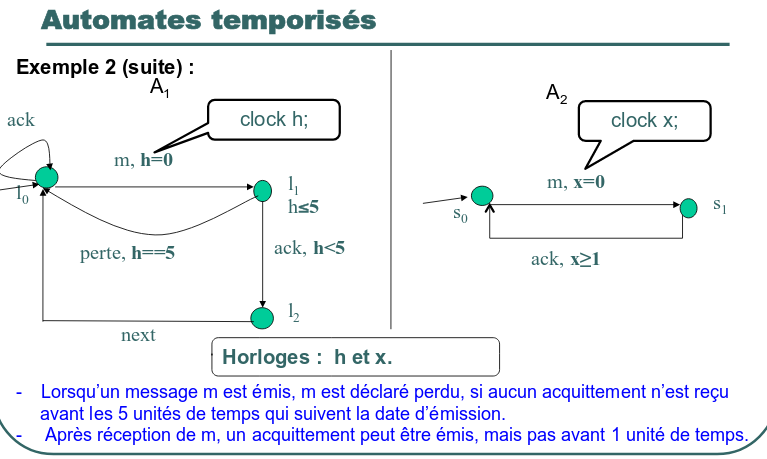
\includegraphics[width = 7cm, height = 7cm, keepaspectratio]{Images/automate_temporise.png}
    	\caption{L'automate composé sous forme d'automate temporisés}
    	\label{fig:AutomateTemporise}
    \end{figure}
    
    Il suffit d'imposer des contraintes sur les horloges pour modéliser les aspect temporelles des automates.\\
    
    Noter que d'avoir un horloge sur un état signifie qu'on a une contrainte pour rester dans un état. l'absence d'horloge signifie qu'il n'y a aucune limites de temps.\\
    
    Une évolution d'un automate temporisé est une séquence alterné d'états et d'actions continues-discrètes.\\
    
    \begin{figure}[!ht]
    	\centering
    	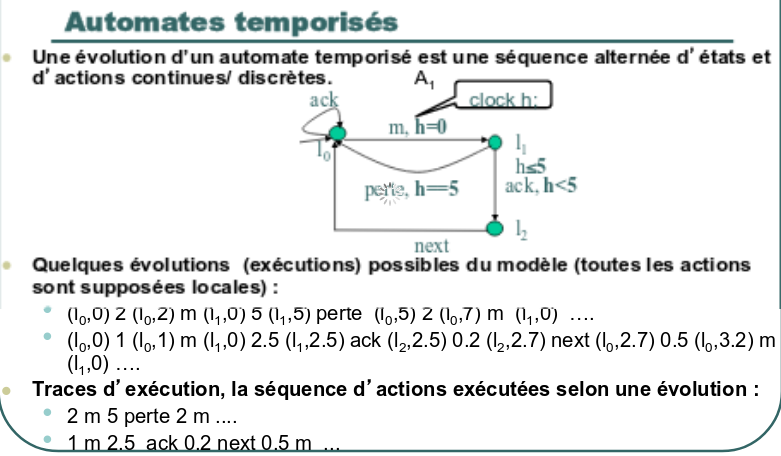
\includegraphics[width = 7cm, height = 7cm, keepaspectratio]{Images/slide15.png}
    	\label{fig:slide15}
    \end{figure}
    
    On peut définir une contrainte temporelle par la grammaire de la slide 16\\
    
    ou x et y sont des horloge, c est un entier et $\angle$$\in$\{$\le$, $\leq$\}\\
    \begin{figure}[!ht]
    	\centering
    	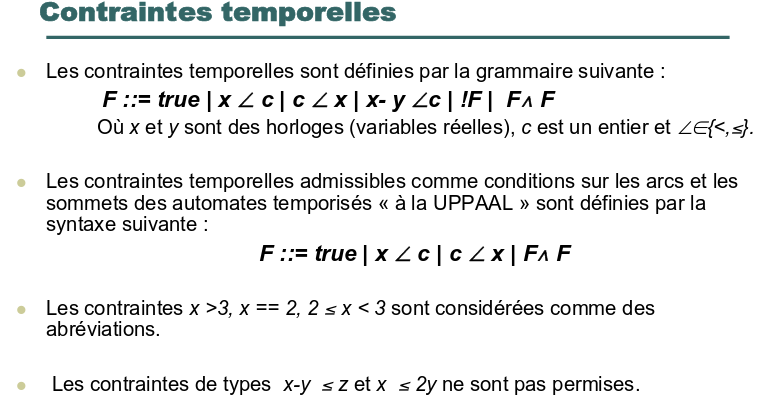
\includegraphics[width = 7cm, height = 7cm, keepaspectratio]{Images/slide16.png}
    	\label{fig:slide16}
    \end{figure}
    
    
    \subsection{Contraintes temporelles}
    Soit un ensemble fini d'horloge\\
    
    une valuation v de H est une fonction qui associe à chaque horloge de H une valeur réelle positive ou nulle. $R^{+}$.\\
    
    soit F une contrainte temporelle sur H et v une valuation de H, dh $\in$ $R^+$ et $H' \in H $\\
    
    \begin{itemize}
    	\item f(v) représente la valeur de vérité de f pour v. v satisfait la condition f ssi f(v) est vraie.
    	\item f est dite consistante satisfiable ssi il existe une valuation de H qui satisfait f.
    \end{itemize}
       
    Soit H un ensemble fini d'horloge, f une contrainte temporelle sur H, v une valuation de H, dh $\in$ $R^+$ et $H' \subseteq H$
    \begin{itemize}
    	\item on désigne la valuation v+dh la valuation définie par : \\
    	$\forall$x $\in$ H, (v + dh)(x) = v(x) + dh
    	\item v[H'= 0] est la valuation obtenue en remplaçant la valeur de chaque horloge de H' par 0.
    	\item on désigne par f[H'=0] la formule obtenue en éliminant par substitution les horloges de H' et en ajoutant ensuite la contrainte x=0, pour toute horloge x de H'.
    \end{itemize}
    
    \subsubsection{Exemple}
    
    \begin{itemize}
        \item 
        \textbf{f1 est-elle consistante?} \\
        Le contraintes sont rencontrés dans f1 et f2. Alors c'est consistant\\
         v(x) = v(y) = 2\\
         v(x) = v(y) = v(2) = 2
         
        \item 
        \textbf{Donnez la représentation graphique}\\
         x est compris parmis les bornes. On doit faire les contraintes vertical/horizontal pour x et y. On rajoute ensuite les contraintes diagonale.\\
         
        
        
        
    \end{itemize}
    
    \subsection{Définition et représentation graphique}
    Pour une représentation graphique, on  modifie une condition d'un automate \\
    
    \begin{figure}[!ht]
    	\centering
    	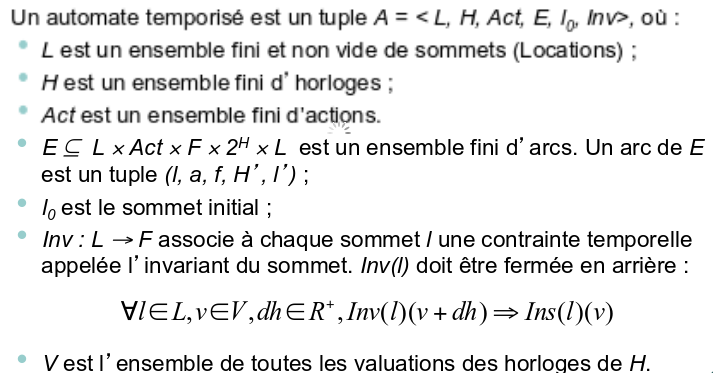
\includegraphics[width = 7cm, height = 7cm, keepaspectratio]{Images/definition_representation_graphique.png}
    	\caption{Définition et représentation graphique}
    	\label{fig:DefinitionRepGraphique}
    \end{figure}

    On défini Inv comme étant l'invariant. Elle associe une contrainte temporelle applée L à chaque sommet. Inv(l) doit être fermée en arrière.\\
    
    $\forall$ $\in$ L, v $\in$V, dH $\in$...\\
    
    Le principe est que certaine formulation d'invariant peuvent donner des comportements inattendus.\\
    
    Un état du modèle est défini par un couple composé d'un sommet I et d'une valuation v des horloges de H qui satisfait Inv(I), i.e.: Inv(l)(v) est vraie.\\
    
    on peut seulement prendre une transition si la valuation de sa transition est vraie.\\
    
    
    
    \subsection{Sémantique opérationelle}    
    
    Un système de transitions est un tuple T <Q, $Q_0$, Et, Rt>\\
    \begin{itemize}
        \item Q est un ensemble non vide d'états
        \item Et est un ensemble d'étiquettes
        \item Rt $\subseteq$ Q x Et x Q est une relation de transitions entre les états
        \item Q0 $\subseteq$ Q est un ensemble d'états initiaux
    \end{itemize}

    \begin{figure}[!ht]
    	\centering
    	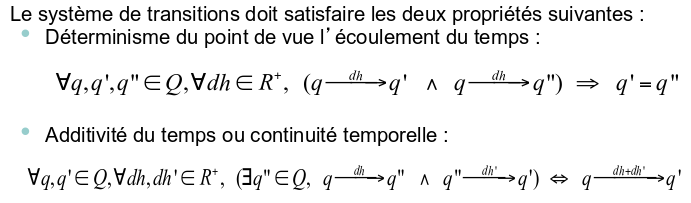
\includegraphics[width = 7cm, height = 7cm, keepaspectratio]{Images/propriete_system_transition.png}
    	\caption{Propriétés d'un système de transition}
    	\label{fig:Systeme transition}
    \end{figure}
    
    Le système de transitions d'un automate temporisé\\
    
    A = <L, H, Act, E, I0, Inv>\\
    
    \begin{figure}[!ht]
    	\centering
    	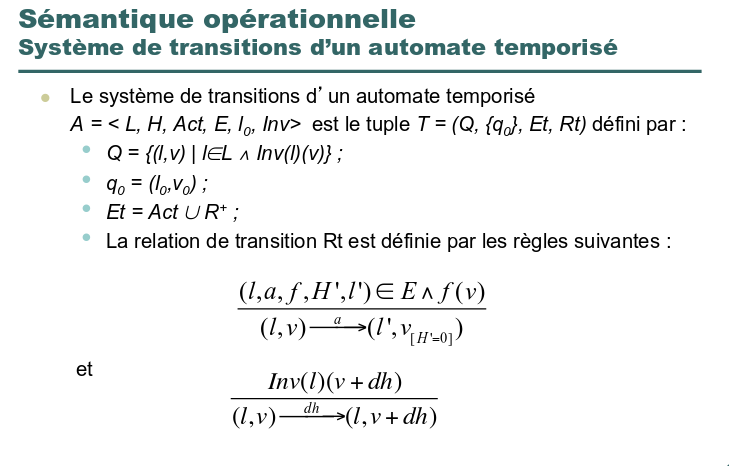
\includegraphics[width = 7cm, height = 7cm, keepaspectratio]{Images/slide28.png}
    	\caption{d'autres propriétés d'un système de transition}
    	\label{fig:Systeme transition2}
    \end{figure}
    
    \begin{figure}[!ht]
    	\centering
    	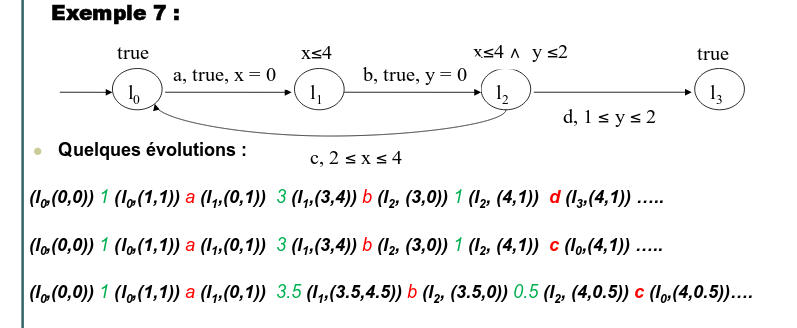
\includegraphics[width = 7cm, height = 7cm, keepaspectratio]{Images/exemple_evolution.png}
    	\caption{Exemple d'Évolution}
    	\label{fig:ExempleEvolution}
    \end{figure}
    
    Note, il n'existe pas d'évolution qui supporte ABA vu que l'invariant de l1 éjecte en dehors de l1 à x$\geq$2\\
    
    \subsection{Automates bien temporisés}
    
    Une évolution inif est à temps divergent si la somme des temps de séjours dans ses locations est infinis, convergent quand ses finis.\\
    
    \subsubsection{Temps convergent et zénon}
    
    la suite peu avoir une infinité d'actions, sauf que l'invariant de on ne supporte pas une valeur d'horloge en haut de 2.\\
    
    Pour un non-zénon, dans tout cycle élémentaire de transitions discrète au moins une horloge est remise à zéro et comparé à une orne inférieur strictement positive.\\
    
    
    un état a un verrou temporel (timelock) si il n'a aucune évolution à temps divergent \\
    
    dans la deuxième image, aucune possibilité d'été pour une valeur de x supérieur à 2\\
    
    Un automate temporisé est à l'état bloqué si aucune action de Act ne peut être exécuté à partir de cet état (état bloqué).\\
    
    un automate est bien temporisé si: pour chaque état accessible q (l,v) il existe une action a de Act ou un réel positif dh tel que \\
    
    et il est non zénon (toutes ses évolutions sont non zénon).
    \section{Composition d'automates temporisé}
    
    \begin{figure}[!ht]
    	\centering
    	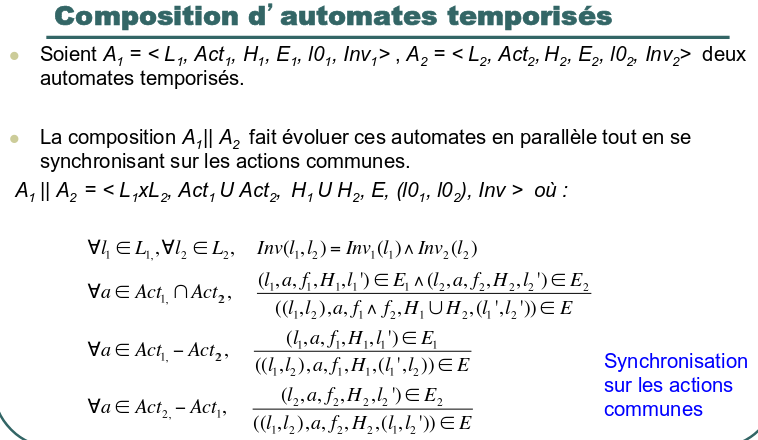
\includegraphics[width = 7cm, height = 7cm, keepaspectratio]{Images/composition_automate_temporise.png}
    	\caption{Propriété d'une composition d'automates temporisé}
    	\label{fig:CompositionAutomateTemporise}
    \end{figure}
    
    On fait comme au début du cours, on fait l'union des actions, horloge et états.. c'est gros.\\
    
    Les composition d'automates se généralise à un ensemble  d'automate..\\
    
    Pour synchroniser deux automates, il faut tout simplement mettre la même actions.\\
    
    
    \section{Automate temporisé à la UPPAAL}
    \section{Automates hybride, à chronomêtre, à couts}
    
\end{document}